%%%%%%%%%%%%%%%%%%%%%%%%%%%%%%%%%%%%%%%%%
% LaTeX Template
%
% This template originates from:
% http://www.LaTeXTemplates.com
%
% License:
% CC BY-NC-SA 3.0 (http://creativecommons.org/licenses/by-nc-sa/3.0/)
% 
%%%%%%%%%%%%%%%%%%%%%%%%%%%%%%%%%%%%%%%%%

%----------------------------------------------------------------------------------------
%	PACKAGES AND OTHER DOCUMENT CONFIGURATIONS
%----------------------------------------------------------------------------------------

\documentclass{article}

%%%%%%%%%%%%%%%%%%%%%%%%%%%%%%%%%%%%%%%%%
% Lachaise Assignment
% Structure Specification File
% Version 1.0 (26/6/2018)
%
% This template originates from:
% http://www.LaTeXTemplates.com
%
% Authors:
% Marion Lachaise & François Févotte
% Vel (vel@LaTeXTemplates.com)
%
% License:
% CC BY-NC-SA 3.0 (http://creativecommons.org/licenses/by-nc-sa/3.0/)
% 
%%%%%%%%%%%%%%%%%%%%%%%%%%%%%%%%%%%%%%%%%

%----------------------------------------------------------------------------------------
%	PACKAGES AND OTHER DOCUMENT CONFIGURATIONS
%----------------------------------------------------------------------------------------

\usepackage{amsmath,amsfonts,stmaryrd,amssymb} % Math packages

\usepackage{enumerate} % Custom item numbers for enumerations

\usepackage[ruled]{algorithm2e} % Algorithms

\usepackage[framemethod=tikz]{mdframed} % Allows defining custom boxed/framed environments

\usepackage{listings} % File listings, with syntax highlighting
\lstset{
	basicstyle=\ttfamily, % Typeset listings in monospace font
}

%----------------------------------------------------------------------------------------
%	DOCUMENT MARGINS
%----------------------------------------------------------------------------------------

\usepackage{geometry} % Required for adjusting page dimensions and margins

\geometry{
	paper=a4paper, % Paper size, change to letterpaper for US letter size
	top=2.5cm, % Top margin
	bottom=3cm, % Bottom margin
	left=2.5cm, % Left margin
	right=2.5cm, % Right margin
	headheight=14pt, % Header height
	footskip=1.5cm, % Space from the bottom margin to the baseline of the footer
	headsep=1.2cm, % Space from the top margin to the baseline of the header
	%showframe, % Uncomment to show how the type block is set on the page
}

%----------------------------------------------------------------------------------------
%	FONTS
%----------------------------------------------------------------------------------------

\usepackage[utf8]{inputenc} % Required for inputting international characters
\usepackage[T1]{fontenc} % Output font encoding for international characters

\usepackage{XCharter} % Use the XCharter fonts

%----------------------------------------------------------------------------------------
%	COMMAND LINE ENVIRONMENT
%----------------------------------------------------------------------------------------

% Usage:
% \begin{commandline}
%	\begin{verbatim}
%		$ ls
%		
%		Applications	Desktop	...
%	\end{verbatim}
% \end{commandline}

\mdfdefinestyle{commandline}{
	leftmargin=10pt,
	rightmargin=10pt,
	innerleftmargin=15pt,
	middlelinecolor=black!50!white,
	middlelinewidth=2pt,
	frametitlerule=false,
	backgroundcolor=black!5!white,
	frametitle={Command Line},
	frametitlefont={\normalfont\sffamily\color{white}\hspace{-1em}},
	frametitlebackgroundcolor=black!50!white,
	nobreak,
}

% Define a custom environment for command-line snapshots
\newenvironment{commandline}{
	\medskip
	\begin{mdframed}[style=commandline]
}{
	\end{mdframed}
	\medskip
}

%----------------------------------------------------------------------------------------
%	FILE CONTENTS ENVIRONMENT
%----------------------------------------------------------------------------------------

% Usage:
% \begin{file}[optional filename, defaults to "File"]
%	File contents, for example, with a listings environment
% \end{file}

\mdfdefinestyle{file}{
	innertopmargin=1.6\baselineskip,
	innerbottommargin=0.8\baselineskip,
	topline=false, bottomline=false,
	leftline=false, rightline=false,
	leftmargin=2cm,
	rightmargin=2cm,
	singleextra={%
		\draw[fill=black!10!white](P)++(0,-1.2em)rectangle(P-|O);
		\node[anchor=north west]
		at(P-|O){\ttfamily\mdfilename};
		%
		\def\l{3em}
		\draw(O-|P)++(-\l,0)--++(\l,\l)--(P)--(P-|O)--(O)--cycle;
		\draw(O-|P)++(-\l,0)--++(0,\l)--++(\l,0);
	},
	nobreak,
}

% Define a custom environment for file contents
\newenvironment{file}[1][File]{ % Set the default filename to "File"
	\medskip
	\newcommand{\mdfilename}{#1}
	\begin{mdframed}[style=file]
}{
	\end{mdframed}
	\medskip
}

%----------------------------------------------------------------------------------------
%	NUMBERED QUESTIONS ENVIRONMENT
%----------------------------------------------------------------------------------------

% Usage:
% \begin{question}[optional title]
%	Question contents
% \end{question}

\mdfdefinestyle{question}{
	innertopmargin=1.2\baselineskip,
	innerbottommargin=0.8\baselineskip,
	roundcorner=5pt,
	nobreak,
	singleextra={%
		\draw(P-|O)node[xshift=1em,anchor=west,fill=white,draw,rounded corners=5pt]{%
		Question \theQuestion\questionTitle};
	},
}

\newcounter{Question} % Stores the current question number that gets iterated with each new question

% Define a custom environment for numbered questions
\newenvironment{question}[1][\unskip]{
	\bigskip
	\stepcounter{Question}
	\newcommand{\questionTitle}{~#1}
	\begin{mdframed}[style=question]
}{
	\end{mdframed}
	\medskip
}

%----------------------------------------------------------------------------------------
%	WARNING TEXT ENVIRONMENT
%----------------------------------------------------------------------------------------

% Usage:
% \begin{warn}[optional title, defaults to "Warning:"]
%	Contents
% \end{warn}

\mdfdefinestyle{warning}{
	topline=false, bottomline=false,
	leftline=false, rightline=false,
	nobreak,
	singleextra={%
		\draw(P-|O)++(-0.5em,0)node(tmp1){};
		\draw(P-|O)++(0.5em,0)node(tmp2){};
		\fill[black,rotate around={45:(P-|O)}](tmp1)rectangle(tmp2);
		\node at(P-|O){\color{white}\scriptsize\bf !};
		\draw[very thick](P-|O)++(0,-1em)--(O);%--(O-|P);
	}
}

% Define a custom environment for warning text
\newenvironment{warn}[1][Warning:]{ % Set the default warning to "Warning:"
	\medskip
	\begin{mdframed}[style=warning]
		\noindent{\textbf{#1}}
}{
	\end{mdframed}
}

%----------------------------------------------------------------------------------------
%	INFORMATION ENVIRONMENT
%----------------------------------------------------------------------------------------

% Usage:
% \begin{info}[optional title, defaults to "Info:"]
% 	contents
% 	\end{info}

\mdfdefinestyle{info}{%
	topline=false, bottomline=false,
	leftline=false, rightline=false,
	nobreak,
	singleextra={%
		\fill[black](P-|O)circle[radius=0.4em];
		\node at(P-|O){\color{white}\scriptsize\bf i};
		\draw[very thick](P-|O)++(0,-0.8em)--(O);%--(O-|P);
	}
}

% Define a custom environment for information
\newenvironment{info}[1][Info:]{ % Set the default title to "Info:"
	\medskip
	\begin{mdframed}[style=info]
		\noindent{\textbf{#1}}
}{
	\end{mdframed}
}
 % Include the file specifying the document structure and custom commands

\usepackage{graphicx}
%Path in Windows format:
\graphicspath{ {.Images/} }

%----------------------------------------------------------------------------------------
%	ASSIGNMENT INFORMATION
%----------------------------------------------------------------------------------------

\title{Gambler's Ruin - Theory} % Title of the assignment

\author{Tansel Arif\\ \texttt{tanselarif@live.co.uk}} % Author name and email address

\date{\today} % University, school and/or department name(s) and a date

%----------------------------------------------------------------------------------------

\begin{document}

\maketitle % Print the title

%----------------------------------------------------------------------------------------
%	INTRODUCTION
%----------------------------------------------------------------------------------------

\section*{Introduction} % Unnumbered section

The Gambler's Ruin problem frames a gambler who begins gambling with an initial fortune - in dollars say. At each successive gamble, the gambler either loses \$1 or gains \$1. The problem is to find the probability that the gambler goes bankrupt - loses the entirety of the fortune. This problem is a kind of random walk. Figures \ref{fig:sim1} and \ref{fig:sim2} below show simulation trajectories for this setup.

\begin{figure}[r]
    \centering
    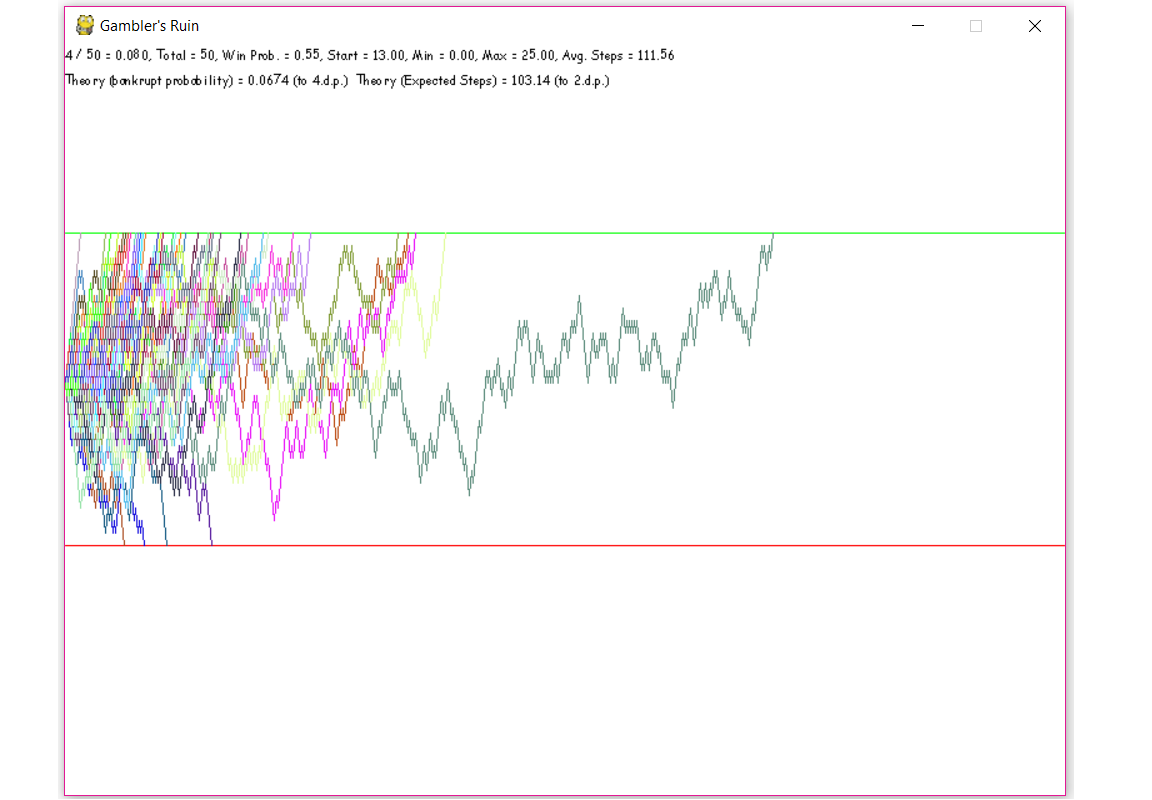
\includegraphics[width=\textwidth]{Simulation1}
    \caption{This is a plot of 10 simulations with $k = 12.5$, $p = 0.55$, $N = 25$. The theory results in a probability of 0.0753 of bankruptcy. The horizontal green line represents \$N and the hosrizontal red line represents \$0.}
    \label{fig:sim1}
\end{figure}

\begin{figure}[r]
    \centering
    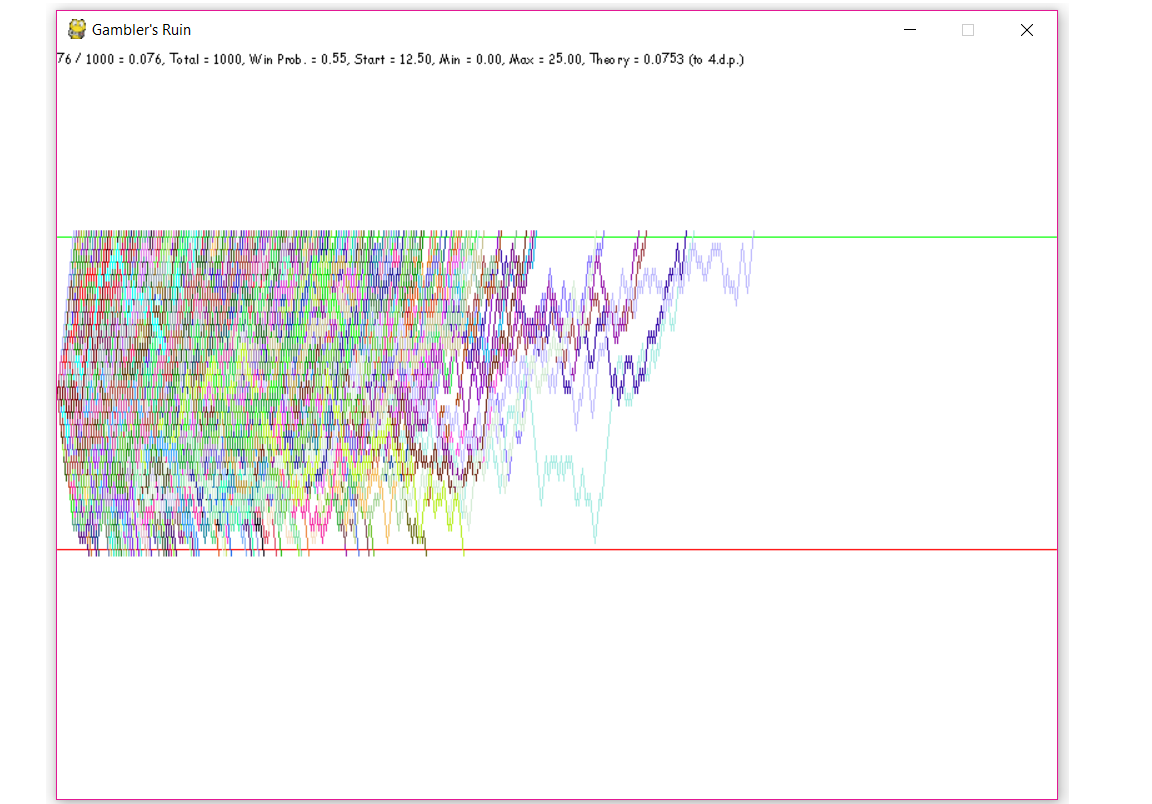
\includegraphics[width=\textwidth]{Simulation2}
    \caption{This is a plot of 1000 simulations with $k = 12.5$, $p = 0.55$, $N = 25$. The theory results in a probability of 0.0753 of bankruptcy. The horizontal green line represents \$N and the hosrizontal red line represents \$0.}
    \label{fig:sim2}
\end{figure}

\section{The Problem} % Numbered section

A Gambler begins with \$k and repeatedly plays a game after which they may win \$1 with probability $p$ or lose \$1 with probability $q=1-p$. The Gambler will stop playing if their fortune reaches \$0 or \$N. What is the probability that they go bankrupt?

\section{The Solution} % Numbered section

Let $u_k$ be the probability that the Gambler bankrupts if the initial fortune is \$k. Then we can condition this probability on the first gamble as follows (utilising the law of total probability with the partitioning of lose/win):

$$u_k = P(wins) \times u_{k+1} + P(loses) \times u_{k-1}$$

This is a second order homogeneous difference equation. We look for solutions of the form $u_n = A \times \lambda^n$.

$$p \times u_{n+1} - u_n + q u_{n-1} = 0$$
$$\implies p \times A \times \lambda^{n+1} - A \times \lambda^n + q \times A \times \lambda^{n-1} = 0$$
$$\implies \lambda^{2} - \frac{1}{p} \lambda + \frac{q}{p} = 0$$

where $p, q \neq 0$. This has solution:

$$\lambda_{1,2} = \left\{\frac{1-p}{p},1\right\}$$

provided that $p \neq \frac{1}{2}$, this gives 2 different solutions. We have:

$$u_n = A \left( \frac{1-p}{p} \right)^n + B (1)^n$$
$$ = A \left( \frac{1-p}{p} \right)^n + B$$

We have that the Gambler stops gambling if either their fortune reaches \$0 or \$N. So we have the following boundary conditions:

$$u_0 = 1, u_N = 0$$

Using these boundary conditions, we can solve for $A$ and $B$:

$$u_0 = A \left( \frac{1-p}{p} \right)^0 + B = 1$$
$$\implies A+B = 1$$
$$\implies B = 1 - A$$

and

$$u_N = A \left( \frac{1-p}{p} \right)^N + B = 0$$
$$\implies B = -A \left( \frac{1-p}{p} \right)^N$$
$$\implies 1 - A = -A \left( \frac{1-p}{p} \right)^N$$
$$\implies A = \frac{1}{1 - \left( \frac{1-p}{p} \right)^N}$$
$$\implies B = 1-A = \frac{-\left( \frac{1-p}{p} \right)^N}{1 - \left( \frac{1-p}{p} \right)^N}$$

Giving the final solution:

\begin{equation}
    u_n = \frac{\left( \frac{1-p}{p} \right)^n-\left( \frac{1-p}{p} \right)^N}{1 - \left( \frac{1-p}{p} \right)^N}
\end{equation}

For the case where $p = \frac{1}{2}$, we try the next most complex expression, let:

$$u_n = (An + B) \times \lambda^n$$

with $\lambda = 1$:

$$u_n = (An + B)$$

We can try this in the original equation with $p=q=1/2$:

$$\frac{1}{2} u_{n+1} - u_n + \frac{1}{2} u_{n-1} = \frac{An}{2} + \frac{A}{2} + \frac{B}{2} - An -B + \frac{An}{2} - \frac{A}{2} + \frac{B}{2} = 0$$

Using the boundary conditions:

$$u_0 = B = 1$$

$$u_N = AN + B = 0 \implies A = \frac{-1}{N}$$

Giving the final equation as:

\begin{equation}
    u_n = 1 - \frac{n}{N}
\end{equation}

We have the final equations for the probability of bankruptcy as:

\begin{equation}
   u_n=% 
   \begin{cases}
     1 - \frac{n}{N} &\text{if $p = 0.5$} \\
     \frac{\left( \frac{1-p}{p} \right)^n-\left( \frac{1-p}{p} \right)^N}{1 - \left( \frac{1-p}{p} \right)^N} &\text{if $p \neq 0.5$ and $p \neq 0$} \\
     1 &\text{if $p = 0$}
   \end{cases}
\end{equation}

Note: The case where $p=0$ is obtained by multiplying the numerator and denominator of the $p\neq 0.5$ case by $p^N$ and simplifying.

\section{Expected Number of Steps} % Numbered section

We can now ask the question "How many times is the Gambler expected to be able to gamble until he stops?". We can approach the solution in a similar manner as the probability calculation in the previous section. Namely, conditioning on the first gamble.

Let $E_n$ be the expected number of steps until the Gambler's fortune reaches either \$0 or \$N if the fortune starts at \$n. We then condition on the first gamble as follows:

$$Expected Steps from n = p \times (1 + Expected Steps from n+1) + q \times (1 + Expected Steps from n-1) $$
$$E_n = p \times (1 + E_{n+1}) + q \times (1 + E_{n-1}) $$

Re-writing:

$$p \times E_{n+1} - E_n + q \times E_{n-1} = -1$$

Unlike in the previous section, this is a heterogeneous equation. A solution to this equation can be written in the form: $E_n = w_n + v_n$. We first find a solution to the homogeneous equation ($w_n$) and a solution to the heterogeneous equation ($v_n$). 

As before, let $w_n = A \lambda^n$, where $A$ is a constant. We have:

$$p w_{n+1} - w_n + q w_{n-1} = 0$$
$$\implies \lambda^2 - \frac{1}{p} \lambda + \frac{q}{p} = 0$$

Giving solutions:

$$\lambda_{1,2} = (\frac{q}{p}, 1)$$

Our solution to the homogeneous equation is then:

$$w_n = A \lambda_1^n + B \lambda_2^n = A (\frac{q}{p})^n + B$$

For a particular solution ($v_n$) to the heterogeneous equation we try $v_n = Cn$:

$$p C(n+1) - Cn + q C(n-1) = -1 $$
$$\implies pC - qC = -1$$

Giving:

$$C = \frac{-1}{p-q}$$

and our particular solution is 

$$v_n = \frac{-n}{p-q}$$

Giving the full solution as

\begin{equation}
    E_n = w_n + v_n = A (\frac{q}{p})^n + B - \frac{n}{p-q} 
\end{equation}

Using the boundary conditions $E_0 = 0, E_N = 0$

$$E_0 = A + B = 0 \implies B = -A$$

$$E_N = A (\frac{q}{p})^N + B - \frac{N}{p-q} = 0$$
$$\implies A((\frac{q}{p})^N - 1) = \frac{N}{p-q}$$
$$\implies A = \frac{N}{(p-q)((\frac{q}{p})^N - 1)}$$

Our final solution is then (for $p \neq \frac{1}{2}$)

\begin{equation}
    E_n = \frac{N}{(p-q)((\frac{q}{p})^N - 1)} (\frac{q}{p})^n - \frac{N}{(p-q)((\frac{q}{p})^N - 1)} - \frac{n}{p-q} 
\end{equation}

Suppose $p = \frac{1}{2}$. We get a repeated solution $\lambda = 1$, meaning we try the next most complicated solution to the homogeneous equation

$$w_n = (An+B) \lambda^n = (An+B)$$

For the particular solution to the equation

$$E_{n+1} - 2 E_n + E_{n-1} = -2$$

we try $v_n = Cn^2$ as the next most complicated particular solution. Substituting this into the heterogeneous equation above

$$C(n+1)^2 - 2Cn^2 + C(n-1)^2 = -1$$

giving 

$$C = -1$$

The full equation is then

$$E_n = w_n + v_n = An + B - n^2$$

Applying the boundary conditions

$$E_0 = B = 0$$

$$E_N = AN - N^2 = 0 \implies A = N$$

Giving the final equation for $E_n$

\begin{equation}
    E_n = w_n + v_n = Nn - n^2 
\end{equation}

In summary

\begin{equation}
   E_n=% 
   \begin{cases}
     Nn - n^2 &\text{if $p = 0.5$} \\
     \frac{N}{(p-q)((\frac{q}{p})^N - 1)} (\frac{q}{p})^n - \frac{N}{(p-q)((\frac{q}{p})^N - 1)} - \frac{n}{p-q}  &\text{if $p \neq 0.5$ and $p \neq 0$} \\
     n &\text{if $p = 0$}
   \end{cases}
\end{equation}

Note: The case where $p=0$ is obtained by multiplying the numerator and denominator of the first to terms in the equation for the $p\neq 0.5$ case by $p^N$ and simplifying.

\section{Simulations} % Numbered section

Simulations are carried out using the accompanying Python app utilising Pygame for visualisation. 

It is expected that if the win probability is 1 ($p=1$), the probability of the Gambler going bankrupt should be 0 and the expected number of steps should be the number of steps required to go from the current fortune to \$N. This can be seen in figure \ref{fig:sim4} where each of the 1000 simulations carried out follow the exact same path. If the the win probability is 0 ($p=0$), then we expect that the probability of the Gambler going bankrupt should be 1 and the expected number of steps should be the number of steps required to go from the current fortune to \$0. This can be seen in figure \ref{fig:sim5} where each of the 1000 simulations carried out follow the exact same path. Two further simulations are carried out with identical parameters but different starting fortunes. Figures \ref{fig:sim3} and \ref{fig:sim6} show that a starting fortune closer to \$0 increases the probability of bankruptcy.

\begin{figure}[r]
    \centering
    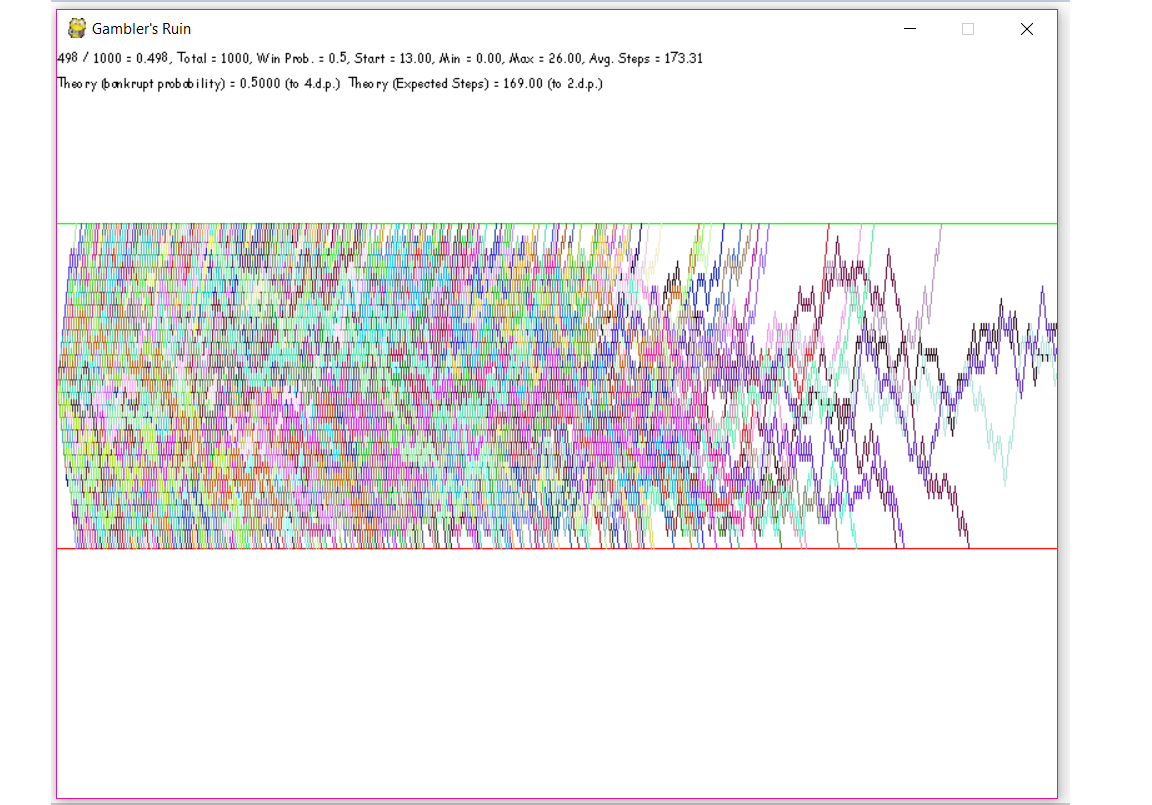
\includegraphics[width=\textwidth]{Simulation3}
    \caption{This is a plot of 1000 simulations with $k = 13$, $p = 0.5$, $N = 26$. The theory results in a probability 0.5 of bankruptcy and an expected number of steps of 169. The horizontal green line represents \$N and the hosrizontal red line represents \$0. We can see that the simulated probability of 0.498 and the simulated average number of steps of 173 is close to the theoretical values.}
    \label{fig:sim3}
\end{figure}

\begin{figure}[r]
    \centering
    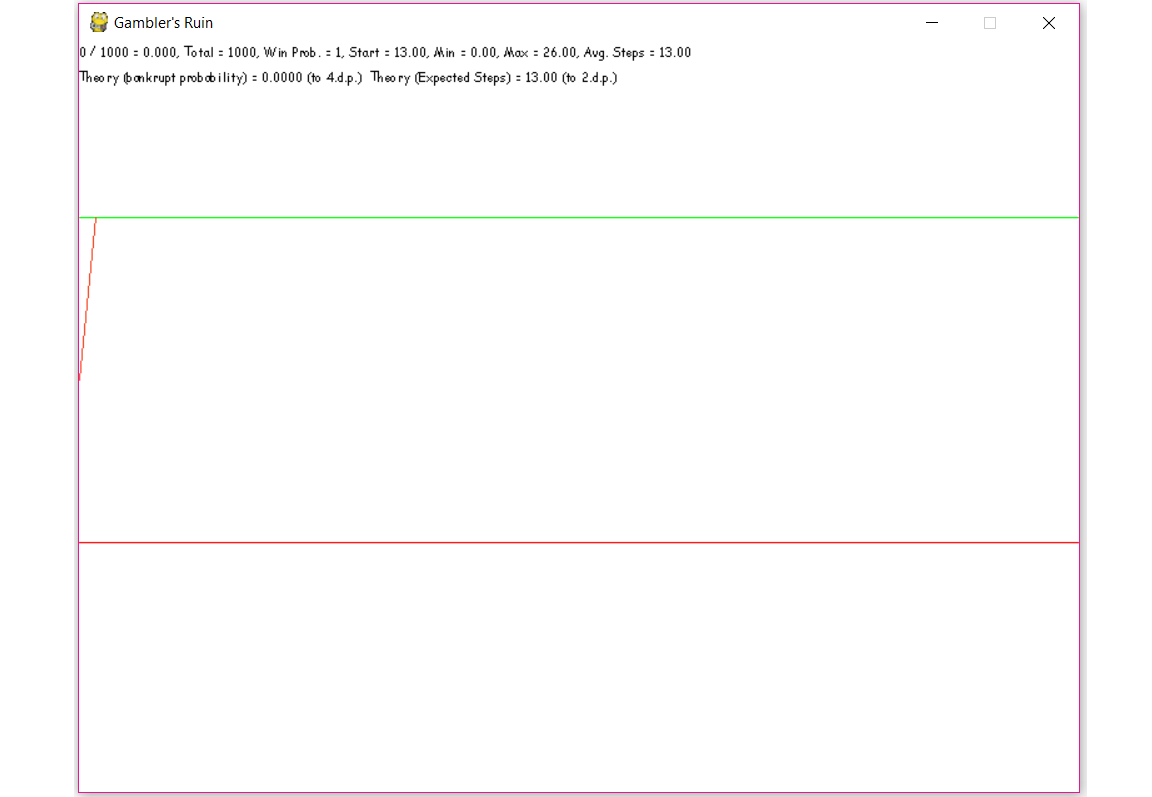
\includegraphics[width=\textwidth]{Simulation4}
    \caption{This is a plot of 1000 simulations with $k = 13$, $p = 1$, $N = 26$. The theory results in a probability 0 of bankruptcy and an expected number of steps of 13. The horizontal green line represents \$N and the hosrizontal red line represents \$0. We can see that the simulated probability of 0 and the simulated average number of steps of 13 exactly match the theoretical values.}
    \label{fig:sim4}
\end{figure}

\begin{figure}[r]
    \centering
    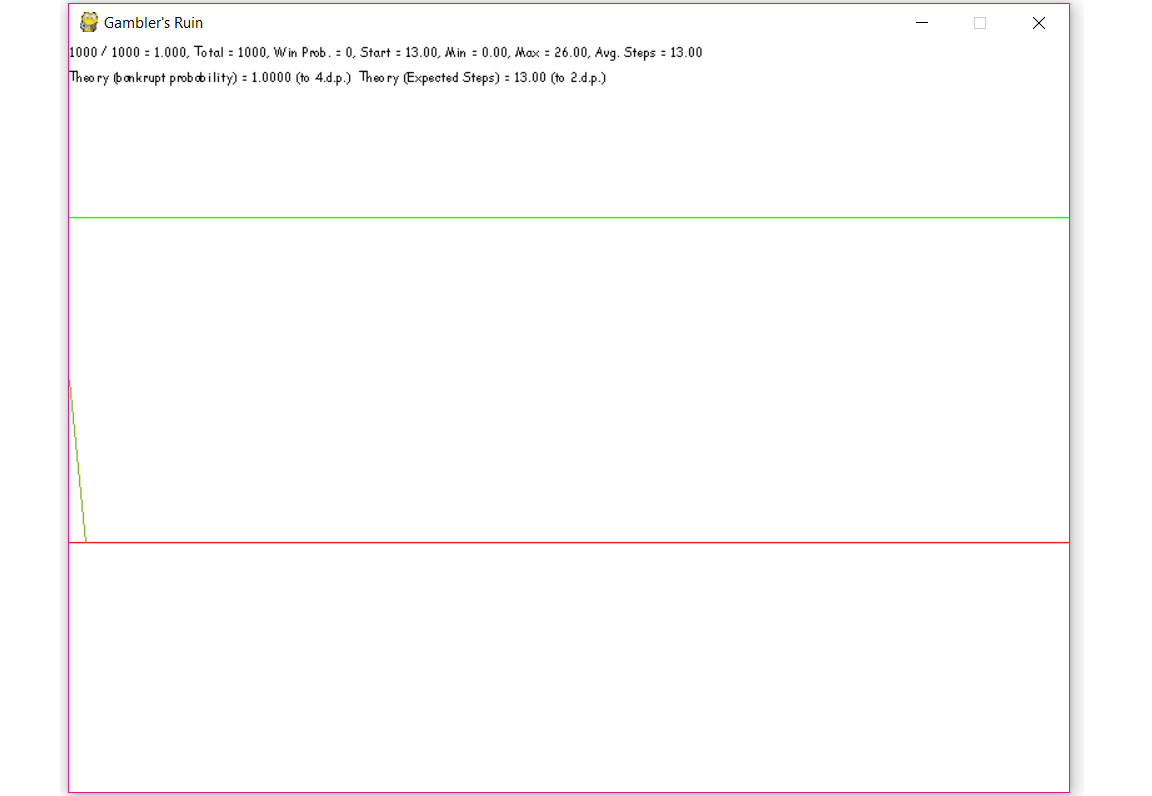
\includegraphics[width=\textwidth]{Simulation5}
    \caption{This is a plot of 1000 simulations with $k = 13$, $p = 0$, $N = 26$. The theory results in a probability 1 of bankruptcy and an expected number of steps of 13. The horizontal green line represents \$N and the hosrizontal red line represents \$0. We can see that the simulated probability of 1 and the simulated average number of steps of 13 exactly match the theoretical values.}
    \label{fig:sim5}
\end{figure}

\begin{figure}[r]
    \centering
    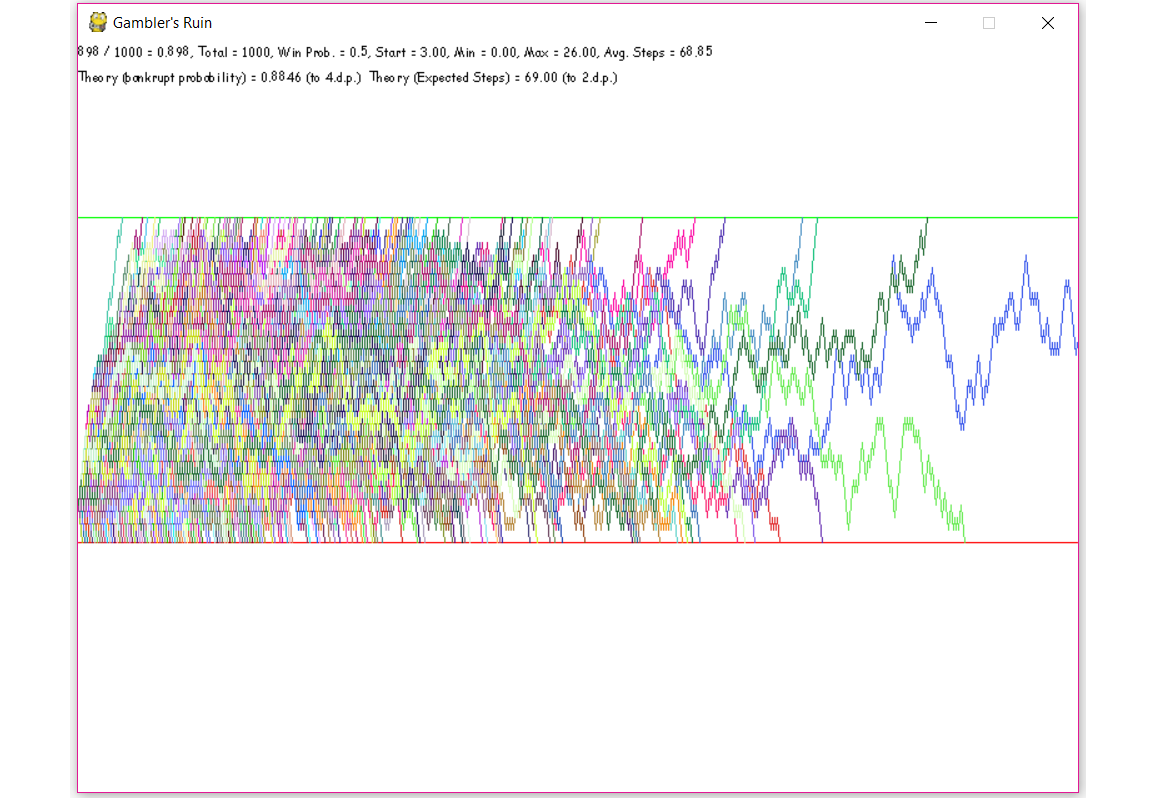
\includegraphics[width=\textwidth]{Simulation6}
    \caption{This is a plot of 1000 simulations with $k = 3$, $p = 0.5$, $N = 26$. The theory results in a probability 0.8846 of bankruptcy and an expected number of steps of 69. The horizontal green line represents \$N and the hosrizontal red line represents \$0. We can see that the simulated probability of 0.898 and the simulated average number of steps of 68.85 match the theoretical values closely.}
    \label{fig:sim6}
\end{figure}

%----------------------------------------------------------------------------------------

\end{document}
